\chapter{Computational Experiments}
\label{chapter:experiments}

We ran computational experiments in two distinct algorithms on instances for the Steiner Multicycle Problem (SMCP). In particular, we implemented the \(3\)-approximation algorithm proposed by \cite{smcp_3apx}, and a relaxed solver to obtain a lower bound to optimal results for the same instances.

It is worth mentioning that we initially tried to run an exact solver to obtain the optimal solutions, but the execution time became prohibitive for this strategy.

# TODO add as footnote
All experiments were executed in an Intel Core i5 11400H with a 16Gb 3200MHz RAM. The code was compiled with Clang version 15.0.1 on a Windows 10 machine. You can see the code at: https://github.com/RaulWCosta/steiner-multicycle-problem-3-apx

The algorithms were implemented in C++ using the Graph library \cite{lemon} and the \cite{gurobi}.

The linear relaxation was implemented using \cite{Pereira2018TheSM} formulation. From \citeauthor{Pereira2018TheSM}, given an instance \((G, c, T)\) of the SMCP, consider a function \(f: 2^V \rightarrow \{0, 1\}\) such that for each non-empty set \(S \subset V\) we have \(f(S) = 1\) if, and only if, there is some \(T_a \in \mathcal{T}\) such that \(S \cap T_a \neq \emptyset\) and \(T_a \nsubseteq S\), i.e., \(S\) is a cut that separates terminals in \(T_a\). They use \(i \in T\) to denote a vertex in a terminal. The SMCP can be formulated as:

\begin{align}
&\text{minimize} &\sum_{e\in E} c_e x_e \label{form-pereira:1}\\
&\text{subject to} &\sum_{e \in \delta(i)} x_e &= 2 &&\text{\(\forall i \in \mathcal{T}\)} \label{form-pereira:2}\\ 
&&\sum_{e \in \delta(S)} x_e &\geq 2 f(S) &&\text{\(\emptyset \neq S \subset V\)} \label{form-pereira:3}\\ 
&&x_e &\in \{0, 1, 2\} &&\text{$e \in E(G)$} \label{form-pereira:4}
\end{align}

Where \(\delta(S)\) denotes the set of edges having exactly one endpoint in \(S\). The variable \(x_e\) indicates if an edge is used in the solution, Constraint~\eqref{form-pereira:2} assures that exactly one cycle covers each terminal, Constraint~\eqref{form-pereira:3} assures that vertices belonging to a terminal set \(T_a \in \mathcal{T}\) are connected, and Constraint~\eqref{form-pereira:4} allows each edge to be used at most twice.

By relaxing the integrality Constraint~\eqref{form-pereira:4} we obtain the linear program used in the implementation. Note that the number of constraints~\eqref{form-pereira:3} is exponential. However, we managed to compute the relaxed LP in polynomial time by using Gomory-Hu trees to solve maximum flow problems between each pair of vertices in the same terminal set \(T_a\). This is the same strategy employed by \cite{Pereira2018TheSM} on their implementations.

# TODO parei aqui

\section{3-approximation Algorithm}

As presented in Section~\ref{subsection:steinermulticycle}, \cite{smcp_3apx} proposed the following algorithm to obtain a 3-approximation for SMCP.

\begin{algorithm}
\caption{SMCP 3-approximation}
\label{algorithm:smcp-3-apx}
\begin{algorithmic}[1]

\Require A complete graph \(G\), a weight function \(w: E(G) \rightarrow \mathbb{Q}_+\) satisfying the triangle inequality, and a partition \(\mathcal{T} = \{T_1, \dots, T_k\}\) of \(V(G)\)

\Ensure A collection \(\mathcal{C}\) of cycles that respects \(\mathcal{T}\)

\State \(r_{i, j} \gets 2\) for every \(i, j \in T_a\) for some \(1 \leq a \leq  k\)
\State \(r_{i, j} \gets 0\) for every \(i \in T_a\) and \(j \in T_b\) for some \(1 \leq a < b \leq k\).
\State \(G' \gets 2ApproxSND(G, w, r)\) \label{alg:3-apx:snd-2-apx}
\State Let \(T\) be the set of odd degree vertices in \(G'\)
\State Let \(w'\) be the restriction of \(w\) to the edges in \(G'\)
\State \(J \gets MinimumTJoin(G', w', T)\) \label{alg:3-apx:t-join}
\State \(H \gets G' + J\)
\State \(\mathcal{C} \gets ShortCutting(H)\) \label{alg:3-apx:shortcutting}
\State return \(\mathcal{C}\)


\end{algorithmic}
\end{algorithm}


% \begin{enumerate}
%     \item Perform a 2-approximation for the Survivable Network Design Problem (SNDP) in \(G\) to find a subgraph \(G'\)
%     \item Calculate a minimum \(T\)-join \(J\) in \(G'\).
%     \item Create an Eulerian graph \(H\) by doubling each edge of \(J\) and adding them to \(G'\).
%     \item Shortcut an Eulerian tour for each component of \(H\) to obtain a collection \(C\) of cycles in \(G\), which is the algorithm's output.

% \end{enumerate}

To calculate the SNDP in line~\eqref{alg:3-apx:snd-2-apx}, we implemented the 2-approximation proposed by \cite{snd-2-apx}. This algorithm solves the linear relaxation of the problem and rounds the solutions. We also used Gomory-Hu trees to add cuts to the linear relaxation at each iteration.

As mentioned by the authors, Theorem~1 from \cite{smcp_3apx} implies that a minimum weight perfect matching in the graph \(G[T]\) weights at most \(w(G')/2\). This means that one can exchange line~\eqref{alg:3-apx:t-join} to compute, instead, a minimum weight perfect matching \(J\) in \(G[T]\). We applied this strategy in our implementation.

The shortcutting in line~\eqref{alg:3-apx:shortcutting} is done by finding any Eulerian cycle within each component of \(H\). We conjecture that the quality of the 3-approximation could be further improved by adopting a better strategy for shortcutting, at the cost of a potentially greater execution time.

\section{Instances}

As of the time of writing, the only experimental study available for the SMCP (more specifically, its restricted version R-SMCP) was the one presented by \cite{Pereira2018TheSM}. In their work, they evaluated implementations of their proposed algorithm and a well-known metaheuristic using two instance types. Type 1 is a set of instances from the multi-commodity one-to-one pickup-and-delivery traveling salesman problem (m-PDTSP), and type 2 is a set of randomly generated instances created by them.

\cite{HERNANDEZPEREZ2009987} generated a set of instances to the m-PDTSP. For each instance, they generated \(2n - 2\) uniformly random points with coordinates from \(-500\) to \(500\), a vertex in position \(0\) with coordinates \((0, 0)\) and a vertex in position \(2n - 1\) also with coordinates \((0, 0)\) (corresponding to Class 3 of \cite{HERNANDEZPEREZ2009987}). Like \cite{Pereira2018TheSM}, we only consider the vertex distribution of these instances. For each \(i \in \{0, \dots, n - 1\}\), we assign a vertex \(i\) as a pickup point of an agent and \(i + n\) as its corresponding delivery point. The instances have 6, 11, and 16 agents, totaling 210 instances. This set of instances is of the type 1.

\cite{Pereira2018TheSM} generated a set of instances having 16, 32, 64, 128, and 256 agents, where vertices correspond to points distributed in a square of dimensions \(100000\) by \(100000\). The square is divided into \(1 \times 1\), \(2 \times 2\), \(3 \times 3\), \(4 \times 4\), and \(5 \times 5\) frames, and each pair of pickup and delivery is in the same frame. The space between frames, which we call a wall, has \(0\%\), \(10\%\), \(20\%\), \(30\%\), or \(40\%\) of the frame’s size. The wall can be seen as a rectangle separating the different frames (see Figure~\ref{fig:instances_type_2}). Notice that there is no wall for the instances with division \(1 \times 1\). The location of each point is chosen uniformly at random. For each combination of the number of agents, frames, and wall size, three instances were generated with different seeds, therefore, 315 instances of type 2 were generated.

\begin{figure}[H]
    \centering
    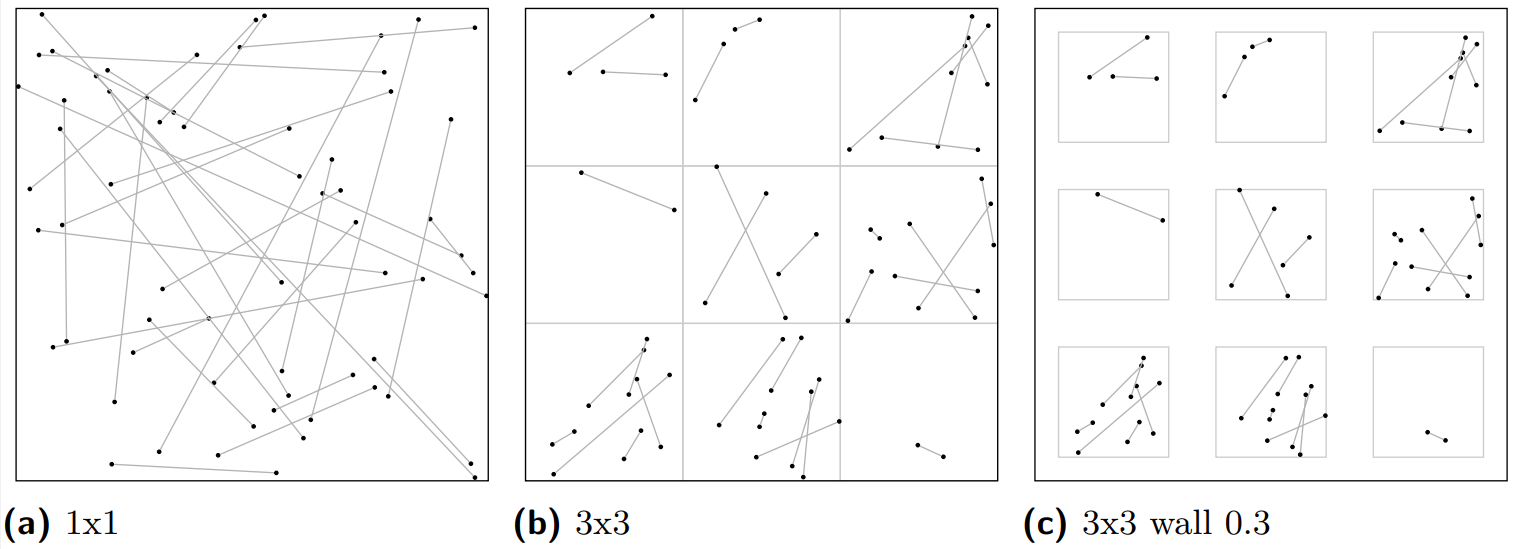
\includegraphics[scale=0.5]{imgs/instances_type_2.png}
    \caption{Instances randomly generated with 16 agents, in (a) a 1 x 1 frame with no wall, in (b) a 3 x 3 frame with \(0\%\) wall, and in (c) a 3 x 3 frame with \(30\%\) wall.}
    \label{fig:instances_type_2}
\end{figure}

\section{Computational Results}

A summary of the experiment results broken by instance group can be seen in Table~\ref{table_avg_apx}. The table shows the gap between the result achieved by the 3-approximation and the linear relaxation, as well as its respective execution times. The first line of the table shows the average results from the type 1 instances. The remaining table sub-divides the type 2 instances depending on some properties. The ``\(1 \times 1\)'' class contains results with a single frame, while the ``\(2 \times 2\)'' class contains the results of the instances with 4 frames, etc. The ``\(W0.x\)'' class contains the results of the instances with wall separation of \((10 \times x)\%\) of the size of the frame (as illustrated in the Figure~\ref{fig:instances_type_2} (c)). The last lines of the table separate the instances by the number of ``agents'' (which is how \citeauthor{Pereira2018TheSM} call terminal pairs).

\begin{table}[H]
\caption{Summary of results by class.}
\centering
    \begin{tabular}{lrrrr}
        \toprule
        Classes & num Inst & GAP (\%) & APX time (s) & relaxed solver time (s) \\
        \midrule
        m-PDTSP & 210 & 33.80 & 0.00 & 0.00 \\
        \hline
        1 $\times$ 1 & 15 & 41.06 & 159.34 & 0.09 \\
        2 $\times$ 2 & 75 & 40.67 & 46.45 & 0.09 \\
        3 $\times$ 3 & 75 & 36.46 & 45.01 & 0.10 \\
        4 $\times$ 4 & 75 & 32.89 & 64.33 & 0.09 \\
        5 $\times$ 5 & 75 & 30.77 & 100.85 & 0.09 \\
        \hline
        W0.0 & 75 & 36.90 & 145.25 & 0.09 \\
        W0.1 & 60 & 37.78 & 109.89 & 0.09 \\
        W0.2 & 60 & 35.36 & 55.96 & 0.09 \\
        W0.3 & 60 & 33.09 & 7.33 & 0.09 \\
        W0.4 & 60 & 32.72 & 5.91 & 0.09 \\
        \hline
        rg-016 & 63 & 23.76 & 0.00 & 0.00 \\
        rg-032 & 63 & 26.02 & 0.03 & 0.00 \\
        rg-064 & 63 & 34.63 & 0.56 & 0.02 \\
        rg-128 & 63 & 36.74 & 12.44 & 0.08 \\
        rg-256 & 63 & 40.98 & 330.44 & 0.35 \\
        \hline
        total average & & 34.21 & 197.10  & 0.29 \\
        \bottomrule
    \end{tabular}
\label{table_avg_apx}
\end{table}


We can see a positive trend between the number of agents (i.e., terminal pairs) and the solution gap. It is also possible to observe a negative trend between the number of frames and the quality of the solution, indicating that the algorithm does not handle well terminal pairs whose terminals are far from each other.

The relationship between the number of terminals in each instance and the optimality gap of the algorithm can be seen in Figure~\ref{fig:hist_opt_gap}. The figure shows that for all instances, the algorithm got significantly closer to the optimality than its 3-approximation guarantee. Although the results, accounting for both execution time and solution quality, were inferior to the heuristic proposed by \cite{Pereira2018TheSM}. 

% \begin{figure}[t!]
%     \centering
%     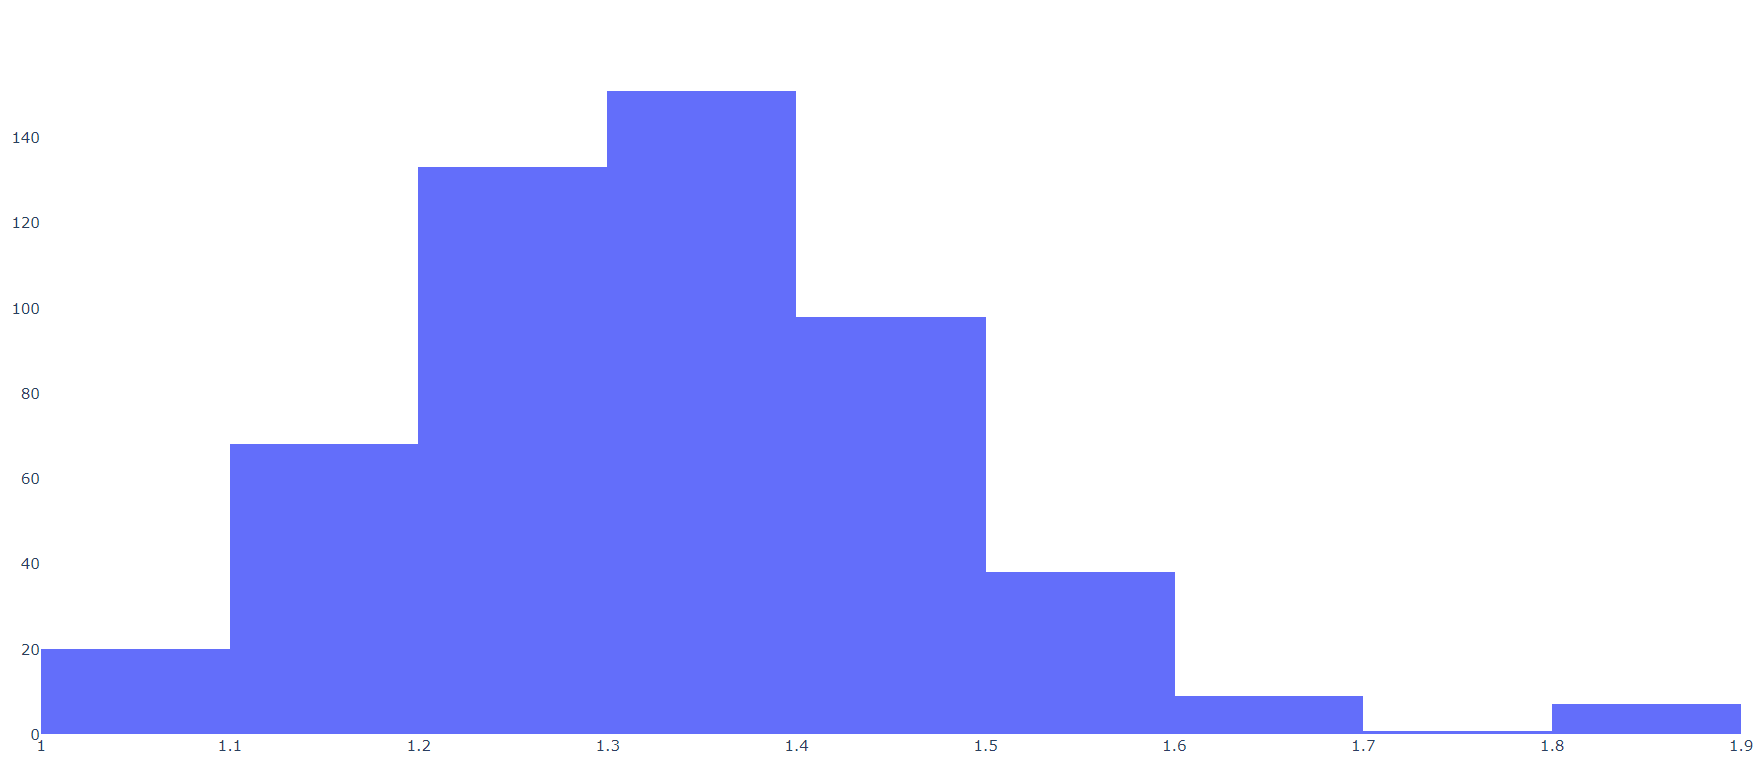
\includegraphics[scale=0.4]{imgs/hist_opt_gap2.png}
%     \caption{Number of instances per optimality gap. An optimality gap of \(1.6\) means that the solution cost is \(60\%\) more than the cost of the relaxation.}
%     \label{fig:hist_opt_gap}
% \end{figure}

\begin{figure}[t!]
\centering
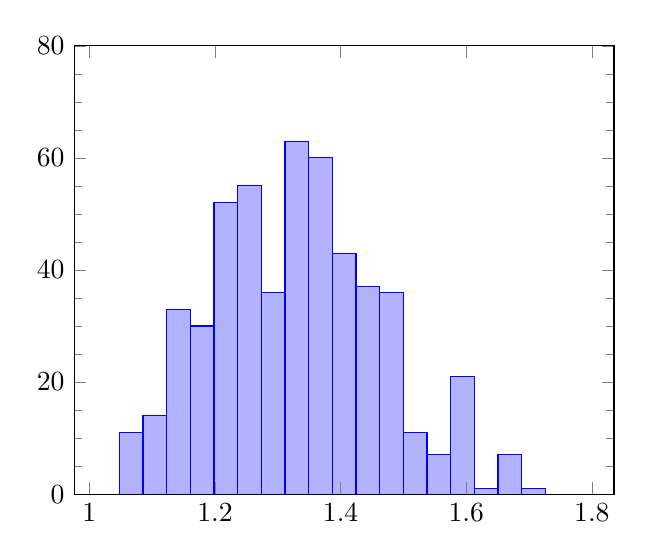
\begin{tikzpicture}
\begin{axis}[
    ymin=0, ymax=80,
    minor y tick num = 3,
    area style,
    ]
\addplot+[ybar interval,mark=no] plot coordinates { (1.0476854749768996, 11) (1.0853661041789102, 14) (1.123046733380921, 33) (1.1607273625829317, 30) (1.1984079917849424, 52) (1.2360886209869533, 55) (1.273769250188964, 36) (1.3114498793909748, 63) (1.3491305085929854, 60) (1.386811137794996, 43) (1.424491766997007, 37) (1.4621723961990176, 36) (1.4998530254010283, 11) (1.5375336546030391, 7) (1.5752142838050498, 21) (1.6128949130070604, 1) (1.6505755422090713, 7) (1.688256171411082, 1) (1.7259368006130926, 0) (1.7636174298151035, 7) };
\end{axis}
\end{tikzpicture}
\caption{Number of instances per optimality gap. An optimality gap of \(1.6\) means that the solution cost is \(60\%\) more than the cost of the relaxation.}
\label{fig:hist_opt_gap}
\end{figure}

Although the algorithm tended to perform better on smaller instances, from the 10 worst performance instances (that is, with the largest gap from the linear relaxation), 9 are from the instances of type 1 containing only 6 terminal pairs.

The implementation of the 3-approximation algorithm executes the shortcut step in line~\eqref{alg:3-apx:shortcutting} by naively finding any Euclidean subgraph contained in each component of the solution; we conjecture that the quality of this algorithm could be improved by applying a more robust shortcutting strategy on the cost of a greater execution time.

In all instances, the time spent to calculate the 2-approximation for the Survivable Network Design Problem accounted for more than \(99\%\) of the total execution time of the algorithm. Moreover, the iterative calculation of Gomory-Hu trees, a step during the solving of the SNDP, has a significant impact on the total execution time, especially for bigger instances, as we can see in Table~\ref{table_gomory_hu_gap}.

\begin{table}[t!]
\caption{Participation of Gomory-Hu trees calculation on total execution time}
\label{table_gomory_hu_gap}
\centering
    \begin{tabular}{lrrrr}
        \toprule
        num vert & num inst & min (\%) & mean (\%) & max (\%) \\
        \midrule
        12 & 70 & 0.00 & 0.00 & 0.00 \\
        22 & 70 & 0.00 & 0.00 & 0.00 \\
        32 & 133 & 0.00 & 0.00 & 0.00 \\
        64 & 63 & 0.00 & 13.63 & 40.90 \\
        128 & 63 & 23.31 & 39.64 & 75.80 \\
        256 & 63 & 30.30 & 51.86 & 78.43 \\
        512 & 63 & 38.68 & 64.89 & 91.76 \\
        \bottomrule
    \end{tabular}
\end{table}

This step might be a good area to improve upon so that the algorithm presents a better execution time in bigger instances.

For practical implementations, a possible alternative would be to use faster heuristics instead of the 2-approximation for the SNDP step (see~\cite{Ker2005}). 
Such heuristics could greatly improve the performance of the algorithm, despite loosing theoretical guarantees of the quality of the solutions.
